\documentclass{article}

\usepackage{listings}
\usepackage{graphicx}
\usepackage{hyperref}
\usepackage{fancyref}

\title{Sorting with Human Intelligence}
\author{Cole Kurashige \\ Harvey Mudd College}
\date{March \\ 2020}

\begin{document}

\maketitle 

\begin{abstract}
  Many comparison-based sorting algorithms have been introduced in years past,
  but none are capable of comparing elements of two different types. We present
  a novel algorithm called Turksort which uses human intelligence to sort lists
  with truly arbitrary contents. We also present an implementation that can be
  found at \url{https://github.com/cole-k/turksort}. We analyze its performance
  with respect to time, accuracy, as well as a novel metric called monetary
  complexity.
\end{abstract}

\section{Background}
Lower bounds for time and space complexity have been long-established for
comparison-based sorting algorithms. Many sorting algorithms have been developed
which vary in the trade-offs they make for these complexities. Little has been
done, however, to examine what it means to make a comparison.

In statically-typed programming languages like Java or C++, comparisons such as
equal to (\texttt{==}) or greater than (\texttt{>}) are often restricted to
operating on two elements of the same type\footnote{At least, without trickery
  or custom comparators.}. These languages consider it a compliation error
to compare elements of differing types.

Dynamically-typed programming languages like Python do not consider it a
compilation error; however, it is usually a runtime error to make these
comparisons.

\begin{lstlisting}[caption = Comparisons in Python 3.7.6]
>>> -1 > '-2'
Traceback (most recent call last):
  File "<stdin>", line 1, in <module>
TypeError: '>' not supported between instances of 'int' and 'str'
\end{lstlisting}

JavaScript, ever the staunch opponent of reason, will gladly compare two objects
of differing types. But just because JavaScript can do something does not mean
that JavaScript does it right.

It will correctly report that \texttt{-1} is greater than \texttt{"-2"}, but it
erroneously considers \texttt{"-1"} less than \texttt{"-2"}. It also doesn't get
that \texttt{"three"} is less than \texttt{"four"}, and it certainly does not
know that \texttt{"one pound of feathers"} is just as heavy as \texttt{"one
  pound of bricks"}.

\begin{lstlisting}[caption = Comparisons in JavaScript (Node.js 12.12.0)]
> -1 > "-2"
true
> "-1" > "-2"
false
> "three" < "four"
false
> "one pound of feathers" == "one pound of bricks"
false
\end{lstlisting}

Though it would be enjoyable to continue to mock JavaScript and its many
questionable design choices, we cannot fault much for these shortcomings.

JavaScript, like any programming language, interprets code. It treats queries
like \texttt{"-1" > "-2"} as being a comparison on characters, not numbers, even
if we humans can plainly see that JavaScript is being asked to compare negative
one and negative two. But we cannot call JavaScript an idiot without calling it
a savant. It can perform remarkably complex calculations in the blink of an eye
or bring the fastest of hardware to a slow grind.

Computers are limited at processing much of the information that is so easy for
us humans to immediately understand, like pictures of dogs or whether
\texttt{"-1"} is greater than \texttt{"-2"}. And we are limited at processing
much of the information that is so easy for computers to understand, like the
exact colors of the millions of pixels in a picture of a dog or the product of
two very large numbers.

\begin{lstlisting}[caption = Complex Operations in JavaScript (Node.js 12.12.0)]
> 0.1 + 0.2
0.30000000000000004
> 1000000000 * 500000000
500000000000000000
\end{lstlisting}

Together, computers and humans can cover for each other's inadequacies, which is
the premise of Human Intelligence Sorting. This type of sorting has yet to been
realized in traditional sorting algorithms. At least until now.

\section{Turksort}

The idea behind turksort is simple: let computers handle all of the sorting
tedium and let humans handle all of the comparisons. It ends up being not that
different from most sorting algorithms.

The algorithm differs only when two values need to be compared. When this
happens, a form asking which of the two is greater\footnote{``Neither'' is an
  option, too.} is generated. This form is sent to Amazon's Mechanical
Turk (MTurk)\footnote{\url{https://www.mturk.com/}} where a worker (known as a
``Turker'') fills it out. The answers is sent back and then used for the
comparison. \Fref{fig:comparison} depicts this process.

\begin{figure}
  \centering
  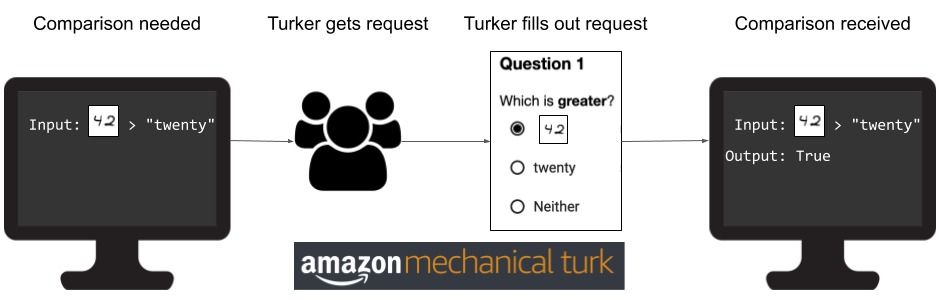
\includegraphics[width=300pt]{diagram-1.png}
  \caption{How Turksort comparisons work}
  \label{fig:comparison}
\end{figure}

An implementation of Turksort is available at
\url{https://github.com/cole-k/turksort}. Any analyses in this paper will be
with reference to this implementation. It is worth noting that Turksort refers
to any algorithm that sorts using Turker-based comparisons, so other variants
may be developed.

The implementation is a modification of quicksort. Quicksort works by selecting
an element in the list (called the ``pivot'') and comparing all of the other
elements to it. It then partitions the list into three groups: those less than,
equal to, or greater than the pivot. It recursively sorts all three partitions
and combines them in order, producing a sorted array.

The paritioning process requires queries to be made comparing the pivot to each
of the other elements in the list. These comparisons are collected and sent to
MTurk for evaluation. This allows us to batch the computations, since querying
MTurk is slow in comparison to regular comparison. The answers from MTurk are
then used in the partitioning, and the algorithm proceeds as usual.

\section{Analysis}

In this section, we analyze the performance of Turksort (\fref{sec:performance})
as well as its accuracy (\fref{sec:accuracy}).

\subsection{Performance}\label{sec:performance}
Turksort is not an algorithm whose performance should be measured by traditional
means. It, however, can be.

Since it retries until it gets a response from the Turker, Turksort technically
has an unbounded time complexity. Even assuming that the response time from the
Turker is bounded and proportionate to the query size, the asymptotic time
complexity is that of quicksort. The average response time, even for shorter
queries, is around 5 minutes, so the constants on the time complexity are very
large.

The novel performance measurement we propose for Turksort is a cost metric. We
call it monetary complexity. This is the asymptotic cost of performing a
computation. Because one currency differs from other currencies by a scaling
factor, the monetary complexity's monetary base does not matter, much like
logarithmic base in asymptotic complexity does not matter. We use a monetary
base of USD.

It takes a Turker about 1 second to answer a single query. Since minimum wage in
California is presently \$ 12.00, we pay 1 cent for every 3 queries a Turker
answers, paying a floor of 1 cent if they are answering fewer than 3. We
measured the monetary complexity of Turksort with respect to the number of
elements in the list, with lists up to size 10000. We calculated the cost as
being the average of five trials. Because the authors do not have any grant
money, testing was done using a simulated Turker.

We introduce a new notation \(\$(f(n))\) to to denote monetary complexity: it
means that a computation has cost asymptotically proportionate to \(f(n)\).
Turksort has a monetary complexity of \(\$(n \log n)\); other common sorting
algorithms have an effective monetary complexity of \(\$(1)\)\footnote{Though
  they cost money by way of using electricity, this is a neglible cost and can
  be considered effectively constant}. You can observe this complexity in
\fref{fig:costs}.

It is evident that Turksort should only be used in cases where traditional
computing does not have sufficient intelligence. The tradeoffs for using
Turksort are both time and money, although common adages suggest that this is
only a single tradeoff. In \fref{sec:future-work} we discuss potential solutions
to these tradeoffs. As it turns out, there is a third, unexpected tradeoff,
which is accuracy. We discuss this below.

\begin{figure}
  \centering
  \includegraphics[width=300pt]{costs.png}
  \caption{The monetary complexity of Turksort plotted for lists of size up to
    10000}
  \label{fig:costs}
\end{figure}

\subsection{Accuracy}\label{sec:accuracy}
Surprisingly, Turksort is not a deterministic algorithm. This is because humans
is not deterministic\footnote{Although it is unknown whether individual humans
  are deterministic, in general no two humans perform comparisons exactly
  alike.}. Not only is Turksort nondeterministic, it is also sometimes wrong.
This is because Turkers do not always perform the right computations. Even on
simple queries, such as \texttt{2 > 3}, they can give an incorrect answer.

This does not mean that Turksort is a useless sorting algorithm. There is a
simple tradeoff between accuracy and speed: the less time a Turker spends
answering a question, the more likely it is to be incorrect. Turksort is already
not winning any races, and that is fine since it serves a specific purpose that
regular sorting algorithms cannot. So making it slightly slower for greater
accuracy is a worthwhile tradeoff. We discuss how to mitigate the problem of
accuracy by making more or slower queries in \fref{sec:future-work}.

\section{Future Work} \label{sec:future-work}
In the previous section, we discussed some limitations of Turksort. In this
section we will discuss how these limitaitons may be overcome.
\Fref{sec:improving-accuracy} discusses ways to improve its accuracy and
\fref{sec:improving-performance} discusses ways to improve its performance.
Turksort is very widely applicable and useful, so we do not need to mention
potential applications or uses.

\subsection{Improving Accuracy}\label{sec:improving-accuracy}

The most important problem Turksort presently faces is an accuracy issue. There
are two potential solutions.

First, Turkers could be forcibly slowed down by imposing a time limit before
they can answer a comparison. This will prevent them from answering so fast that
they get it wrong. The bulk of the time spent waiting in Turksort is in waiting
for a Turker to start responding, so this will not extend the duration of the
algorithm significantly, especially for shorter queries.

Second, Turksort could issue multiple requests for the same query. This way,
majority voting from the Turkers could be used to increase the accuracy. Because
these queries would be sent out in parallel, it is unlikely that this will have
significant impacts on time. This has the additional benefit of making it easier
for Turksort to sort so-called ``trick comparisons,'' like a query of \texttt{"a
  pound of bricks" > "a pound of feathers"}. If, during a computation, a query
is suspected of being a ``trick comparison,'' the algorithm can take the
minority response instead.

\subsection{Improving Performance}\label{sec:improving-performance}

Performance is less important for Turksort, given the time it takes to answer
queries, but as the field of Human Intelligence Sorting grows, faster and
cheaper variants will become more useful. 

One way of improving performance is parallelization. Since queries take a long
time to answer, Turksort could issue multiple queries at once. This can either
be realized by modifying the underlying sorting algorithm to be more parallel,
by making all \({n \choose 2}\) comparison queries at once (thereby increasing
the \(\$(n \log n)\) monetary complexity to \(\$(n^2)\)), or by performing
``branch prediction'' and guessing what the next queries might be.

An obvious way of reducing the monetary complexity is to slow the rate at which
Turkers are rewarded. Though it might seem illegal to not pay Turkers minimum
wage, Turksort does not need to pay its Turkers since the gratification that
they are advancing human progress is payment enough. However, without
large constants, we believe \(\$(1)\) Turksort algorithms to be impossible,
as Turkers are not motivated by this gratification. We are presently exploring
a \(\$(\log^2 n)\) variant of Turksort.

\end{document}